\PassOptionsToPackage{unicode=true}{hyperref} % options for packages loaded elsewhere
\PassOptionsToPackage{hyphens}{url}
%
\documentclass[]{article}
\usepackage{lmodern}
\usepackage{amssymb,amsmath}
\usepackage{ifxetex,ifluatex}
\usepackage{fixltx2e} % provides \textsubscript
\ifnum 0\ifxetex 1\fi\ifluatex 1\fi=0 % if pdftex
  \usepackage[T1]{fontenc}
  \usepackage[utf8]{inputenc}
  \usepackage{textcomp} % provides euro and other symbols
\else % if luatex or xelatex
  \usepackage{unicode-math}
  \defaultfontfeatures{Ligatures=TeX,Scale=MatchLowercase}
\fi
% use upquote if available, for straight quotes in verbatim environments
\IfFileExists{upquote.sty}{\usepackage{upquote}}{}
% use microtype if available
\IfFileExists{microtype.sty}{%
\usepackage[]{microtype}
\UseMicrotypeSet[protrusion]{basicmath} % disable protrusion for tt fonts
}{}
\IfFileExists{parskip.sty}{%
\usepackage{parskip}
}{% else
\setlength{\parindent}{0pt}
\setlength{\parskip}{6pt plus 2pt minus 1pt}
}
\usepackage{hyperref}
\hypersetup{
            pdfborder={0 0 0},
            breaklinks=true}
\urlstyle{same}  % don't use monospace font for urls
\usepackage[margin=1in]{geometry}
\usepackage{graphicx,grffile}
\makeatletter
\def\maxwidth{\ifdim\Gin@nat@width>\linewidth\linewidth\else\Gin@nat@width\fi}
\def\maxheight{\ifdim\Gin@nat@height>\textheight\textheight\else\Gin@nat@height\fi}
\makeatother
% Scale images if necessary, so that they will not overflow the page
% margins by default, and it is still possible to overwrite the defaults
% using explicit options in \includegraphics[width, height, ...]{}
\setkeys{Gin}{width=\maxwidth,height=\maxheight,keepaspectratio}
\setlength{\emergencystretch}{3em}  % prevent overfull lines
\providecommand{\tightlist}{%
  \setlength{\itemsep}{0pt}\setlength{\parskip}{0pt}}
\setcounter{secnumdepth}{0}
% Redefines (sub)paragraphs to behave more like sections
\ifx\paragraph\undefined\else
\let\oldparagraph\paragraph
\renewcommand{\paragraph}[1]{\oldparagraph{#1}\mbox{}}
\fi
\ifx\subparagraph\undefined\else
\let\oldsubparagraph\subparagraph
\renewcommand{\subparagraph}[1]{\oldsubparagraph{#1}\mbox{}}
\fi

% set default figure placement to htbp
\makeatletter
\def\fps@figure{htbp}
\makeatother

\usepackage{hyperref}
\usepackage{graphicx}
\graphicspath{{stat-tables_files/figure-latex/}}
\usepackage{booktabs}
\usepackage{longtable}
\usepackage{array}
\usepackage{multirow}
\usepackage{wrapfig}
\usepackage{float}
\usepackage{colortbl}
\usepackage{pdflscape}
\usepackage{tabu}
\usepackage{threeparttable}
\usepackage{threeparttablex}
\usepackage[normalem]{ulem}
\usepackage{makecell}
\usepackage{xcolor}

\author{}
\date{\vspace{-2.5em}}

\begin{document}

\thispagestyle{empty}
\begin{center}
~\\
\vspace{2cm}
{\Huge Statistical Tables}
~\\~\\
v0.1 (last updated: 15 Mar 2020)
\vspace{5cm}
\end{center}

\begin{center}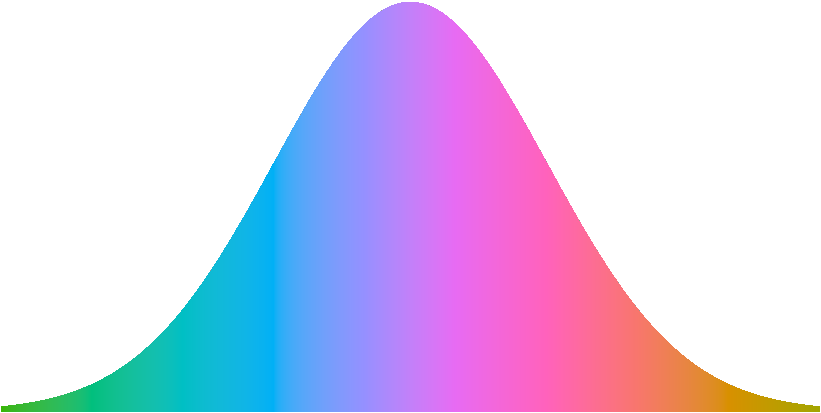
\includegraphics[width=\textwidth]{stat-tables_files/figure-latex/unnamed-chunk-1-1} \end{center}

\vfill
\begin{center}
Copyright (c) 2020 Haziq Jamil
~\\
\href{https://github.com/haziqj/stat-tables}{\texttt{https://github.com/haziqj/stat-tables}}
\end{center}

\newpage

\hypertarget{table-1-cumulative-probabilities-of-the-standard-normal-distribution.}{%
\subsubsection{Table 1: Cumulative probabilities of the standard normal
distribution.}\label{table-1-cumulative-probabilities-of-the-standard-normal-distribution.}}

Each table entry is the area \(A=1-\alpha\) under the standard normal
curve from \(-\infty\) to \(z(\alpha)\).

\vspace{1em}

\begin{center}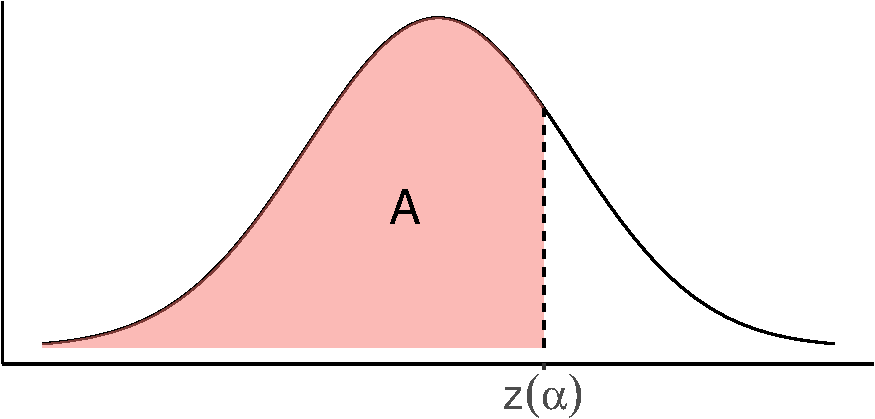
\includegraphics[width=6cm]{stat-tables_files/figure-latex/unnamed-chunk-2-1} \end{center}

\begin{table}[H]
\centering
\begin{tabular}{lrrrrrrrrrr}
\toprule
  & .00 & .01 & .02 & .03 & .04 & .05 & .06 & .07 & .08 & .09\\
\midrule
0.0 & 0.5000 & 0.5040 & 0.5080 & 0.5120 & 0.5160 & 0.5199 & 0.5239 & 0.5279 & 0.5319 & 0.5359\\
0.1 & 0.5398 & 0.5438 & 0.5478 & 0.5517 & 0.5557 & 0.5596 & 0.5636 & 0.5675 & 0.5714 & 0.5753\\
0.2 & 0.5793 & 0.5832 & 0.5871 & 0.5910 & 0.5948 & 0.5987 & 0.6026 & 0.6064 & 0.6103 & 0.6141\\
0.3 & 0.6179 & 0.6217 & 0.6255 & 0.6293 & 0.6331 & 0.6368 & 0.6406 & 0.6443 & 0.6480 & 0.6517\\
0.4 & 0.6554 & 0.6591 & 0.6628 & 0.6664 & 0.6700 & 0.6736 & 0.6772 & 0.6808 & 0.6844 & 0.6879\\
\addlinespace
0.5 & 0.6915 & 0.6950 & 0.6985 & 0.7019 & 0.7054 & 0.7088 & 0.7123 & 0.7157 & 0.7190 & 0.7224\\
0.6 & 0.7257 & 0.7291 & 0.7324 & 0.7357 & 0.7389 & 0.7422 & 0.7454 & 0.7486 & 0.7517 & 0.7549\\
0.7 & 0.7580 & 0.7611 & 0.7642 & 0.7673 & 0.7704 & 0.7734 & 0.7764 & 0.7794 & 0.7823 & 0.7852\\
0.8 & 0.7881 & 0.7910 & 0.7939 & 0.7967 & 0.7995 & 0.8023 & 0.8051 & 0.8078 & 0.8106 & 0.8133\\
0.9 & 0.8159 & 0.8186 & 0.8212 & 0.8238 & 0.8264 & 0.8289 & 0.8315 & 0.8340 & 0.8365 & 0.8389\\
\addlinespace
1.0 & 0.8413 & 0.8438 & 0.8461 & 0.8485 & 0.8508 & 0.8531 & 0.8554 & 0.8577 & 0.8599 & 0.8621\\
1.1 & 0.8643 & 0.8665 & 0.8686 & 0.8708 & 0.8729 & 0.8749 & 0.8770 & 0.8790 & 0.8810 & 0.8830\\
1.2 & 0.8849 & 0.8869 & 0.8888 & 0.8907 & 0.8925 & 0.8944 & 0.8962 & 0.8980 & 0.8997 & 0.9015\\
1.3 & 0.9032 & 0.9049 & 0.9066 & 0.9082 & 0.9099 & 0.9115 & 0.9131 & 0.9147 & 0.9162 & 0.9177\\
1.4 & 0.9192 & 0.9207 & 0.9222 & 0.9236 & 0.9251 & 0.9265 & 0.9279 & 0.9292 & 0.9306 & 0.9319\\
\addlinespace
1.5 & 0.9332 & 0.9345 & 0.9357 & 0.9370 & 0.9382 & 0.9394 & 0.9406 & 0.9418 & 0.9429 & 0.9441\\
1.6 & 0.9452 & 0.9463 & 0.9474 & 0.9484 & 0.9495 & 0.9505 & 0.9515 & 0.9525 & 0.9535 & 0.9545\\
1.7 & 0.9554 & 0.9564 & 0.9573 & 0.9582 & 0.9591 & 0.9599 & 0.9608 & 0.9616 & 0.9625 & 0.9633\\
1.8 & 0.9641 & 0.9649 & 0.9656 & 0.9664 & 0.9671 & 0.9678 & 0.9686 & 0.9693 & 0.9699 & 0.9706\\
1.9 & 0.9713 & 0.9719 & 0.9726 & 0.9732 & 0.9738 & 0.9744 & 0.9750 & 0.9756 & 0.9761 & 0.9767\\
\addlinespace
2.0 & 0.9772 & 0.9778 & 0.9783 & 0.9788 & 0.9793 & 0.9798 & 0.9803 & 0.9808 & 0.9812 & 0.9817\\
2.1 & 0.9821 & 0.9826 & 0.9830 & 0.9834 & 0.9838 & 0.9842 & 0.9846 & 0.9850 & 0.9854 & 0.9857\\
2.2 & 0.9861 & 0.9864 & 0.9868 & 0.9871 & 0.9875 & 0.9878 & 0.9881 & 0.9884 & 0.9887 & 0.9890\\
2.3 & 0.9893 & 0.9896 & 0.9898 & 0.9901 & 0.9904 & 0.9906 & 0.9909 & 0.9911 & 0.9913 & 0.9916\\
2.4 & 0.9918 & 0.9920 & 0.9922 & 0.9925 & 0.9927 & 0.9929 & 0.9931 & 0.9932 & 0.9934 & 0.9936\\
\addlinespace
2.5 & 0.9938 & 0.9940 & 0.9941 & 0.9943 & 0.9945 & 0.9946 & 0.9948 & 0.9949 & 0.9951 & 0.9952\\
2.6 & 0.9953 & 0.9955 & 0.9956 & 0.9957 & 0.9959 & 0.9960 & 0.9961 & 0.9962 & 0.9963 & 0.9964\\
2.7 & 0.9965 & 0.9966 & 0.9967 & 0.9968 & 0.9969 & 0.9970 & 0.9971 & 0.9972 & 0.9973 & 0.9974\\
2.8 & 0.9974 & 0.9975 & 0.9976 & 0.9977 & 0.9977 & 0.9978 & 0.9979 & 0.9979 & 0.9980 & 0.9981\\
2.9 & 0.9981 & 0.9982 & 0.9982 & 0.9983 & 0.9984 & 0.9984 & 0.9985 & 0.9985 & 0.9986 & 0.9986\\
\addlinespace
3.0 & 0.9987 & 0.9987 & 0.9987 & 0.9988 & 0.9988 & 0.9989 & 0.9989 & 0.9989 & 0.9990 & 0.9990\\
3.1 & 0.9990 & 0.9991 & 0.9991 & 0.9991 & 0.9992 & 0.9992 & 0.9992 & 0.9992 & 0.9993 & 0.9993\\
3.2 & 0.9993 & 0.9993 & 0.9994 & 0.9994 & 0.9994 & 0.9994 & 0.9994 & 0.9995 & 0.9995 & 0.9995\\
3.3 & 0.9995 & 0.9995 & 0.9995 & 0.9996 & 0.9996 & 0.9996 & 0.9996 & 0.9996 & 0.9996 & 0.9997\\
3.4 & 0.9997 & 0.9997 & 0.9997 & 0.9997 & 0.9997 & 0.9997 & 0.9997 & 0.9997 & 0.9997 & 0.9998\\
\bottomrule
\end{tabular}
\end{table}

\hypertarget{table-2-percentiles-of-the-chi2-distribution.}{%
\subsubsection{\texorpdfstring{Table 2: Percentiles of the \(\chi^2\)-distribution.}{Table 2: Percentiles of the \textbackslash{}chi\^{}2 distribution.}}\label{table-2-percentiles-of-the-chi2-distribution.}}

Each table entry is \(\chi^2_k(\alpha)\), where
\(\text{P}\big(X < \chi^2_k(\alpha)\big)=A=1-\alpha\) with
\(X\sim\chi^2_k\). \vspace{0.5em}

\begin{center}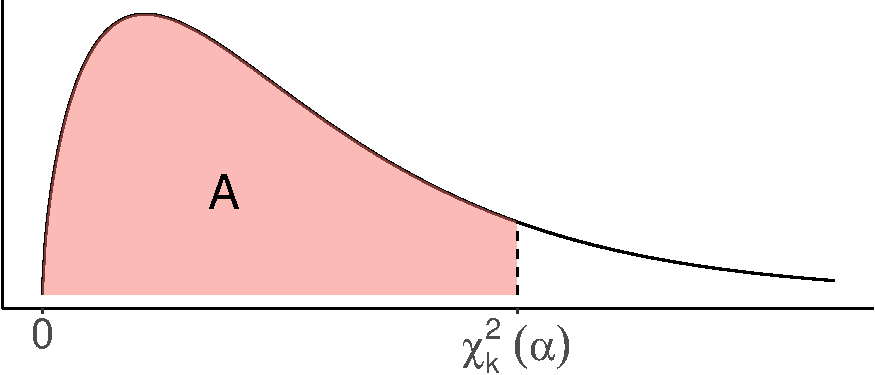
\includegraphics[width=6cm]{stat-tables_files/figure-latex/unnamed-chunk-3-1} \end{center}

\vspace{-0.5em}

\begin{table}[H]
\centering
\begin{tabular}{lrrrrrrrrrr}
\toprule
\multicolumn{1}{c}{ } & \multicolumn{10}{c}{$A$} \\
\cmidrule(l{3pt}r{3pt}){2-11}
$k$ & 0.005 & 0.010 & 0.025 & 0.050 & 0.100 & 0.900 & 0.950 & 0.975 & 0.990 & 0.995\\
\midrule
1 & $0.0^4393$ & $0.0^3157$ & $0.0^3982$ & $0.0^2393$ & 0.016 & 2.706 & 3.841 & 5.024 & 6.635 & 7.879\\
2 & 0.010 & 0.020 & 0.051 & 0.103 & 0.211 & 4.605 & 5.991 & 7.378 & 9.210 & 10.597\\
3 & 0.072 & 0.115 & 0.216 & 0.352 & 0.584 & 6.251 & 7.815 & 9.348 & 11.345 & 12.838\\
4 & 0.207 & 0.297 & 0.484 & 0.711 & 1.064 & 7.779 & 9.488 & 11.143 & 13.277 & 14.860\\
5 & 0.412 & 0.554 & 0.831 & 1.145 & 1.610 & 9.236 & 11.070 & 12.833 & 15.086 & 16.750\\
\addlinespace
6 & 0.676 & 0.872 & 1.237 & 1.635 & 2.204 & 10.645 & 12.592 & 14.449 & 16.812 & 18.548\\
7 & 0.989 & 1.239 & 1.690 & 2.167 & 2.833 & 12.017 & 14.067 & 16.013 & 18.475 & 20.278\\
8 & 1.344 & 1.646 & 2.180 & 2.733 & 3.490 & 13.362 & 15.507 & 17.535 & 20.090 & 21.955\\
9 & 1.735 & 2.088 & 2.700 & 3.325 & 4.168 & 14.684 & 16.919 & 19.023 & 21.666 & 23.589\\
10 & 2.156 & 2.558 & 3.247 & 3.940 & 4.865 & 15.987 & 18.307 & 20.483 & 23.209 & 25.188\\
\addlinespace
11 & 2.603 & 3.053 & 3.816 & 4.575 & 5.578 & 17.275 & 19.675 & 21.920 & 24.725 & 26.757\\
12 & 3.074 & 3.571 & 4.404 & 5.226 & 6.304 & 18.549 & 21.026 & 23.337 & 26.217 & 28.300\\
13 & 3.565 & 4.107 & 5.009 & 5.892 & 7.042 & 19.812 & 22.362 & 24.736 & 27.688 & 29.819\\
14 & 4.075 & 4.660 & 5.629 & 6.571 & 7.790 & 21.064 & 23.685 & 26.119 & 29.141 & 31.319\\
15 & 4.601 & 5.229 & 6.262 & 7.261 & 8.547 & 22.307 & 24.996 & 27.488 & 30.578 & 32.801\\
\addlinespace
16 & 5.142 & 5.812 & 6.908 & 7.962 & 9.312 & 23.542 & 26.296 & 28.845 & 32.000 & 34.267\\
17 & 5.697 & 6.408 & 7.564 & 8.672 & 10.085 & 24.769 & 27.587 & 30.191 & 33.409 & 35.718\\
18 & 6.265 & 7.015 & 8.231 & 9.390 & 10.865 & 25.989 & 28.869 & 31.526 & 34.805 & 37.156\\
19 & 6.844 & 7.633 & 8.907 & 10.117 & 11.651 & 27.204 & 30.144 & 32.852 & 36.191 & 38.582\\
20 & 7.434 & 8.260 & 9.591 & 10.851 & 12.443 & 28.412 & 31.410 & 34.170 & 37.566 & 39.997\\
\addlinespace
21 & 8.034 & 8.897 & 10.283 & 11.591 & 13.240 & 29.615 & 32.671 & 35.479 & 38.932 & 41.401\\
22 & 8.643 & 9.542 & 10.982 & 12.338 & 14.041 & 30.813 & 33.924 & 36.781 & 40.289 & 42.796\\
23 & 9.260 & 10.196 & 11.689 & 13.091 & 14.848 & 32.007 & 35.172 & 38.076 & 41.638 & 44.181\\
24 & 9.886 & 10.856 & 12.401 & 13.848 & 15.659 & 33.196 & 36.415 & 39.364 & 42.980 & 45.559\\
25 & 10.520 & 11.524 & 13.120 & 14.611 & 16.473 & 34.382 & 37.652 & 40.646 & 44.314 & 46.928\\
\addlinespace
26 & 11.160 & 12.198 & 13.844 & 15.379 & 17.292 & 35.563 & 38.885 & 41.923 & 45.642 & 48.290\\
27 & 11.808 & 12.879 & 14.573 & 16.151 & 18.114 & 36.741 & 40.113 & 43.195 & 46.963 & 49.645\\
28 & 12.461 & 13.565 & 15.308 & 16.928 & 18.939 & 37.916 & 41.337 & 44.461 & 48.278 & 50.993\\
29 & 13.121 & 14.256 & 16.047 & 17.708 & 19.768 & 39.087 & 42.557 & 45.722 & 49.588 & 52.336\\
30 & 13.787 & 14.953 & 16.791 & 18.493 & 20.599 & 40.256 & 43.773 & 46.979 & 50.892 & 53.672\\
\addlinespace
40 & 20.707 & 22.164 & 24.433 & 26.509 & 29.051 & 51.805 & 55.758 & 59.342 & 63.691 & 66.766\\
50 & 27.991 & 29.707 & 32.357 & 34.764 & 37.689 & 63.167 & 67.505 & 71.420 & 76.154 & 79.490\\
60 & 35.534 & 37.485 & 40.482 & 43.188 & 46.459 & 74.397 & 79.082 & 83.298 & 88.379 & 91.952\\
70 & 43.275 & 45.442 & 48.758 & 51.739 & 55.329 & 85.527 & 90.531 & 95.023 & 100.425 & 104.215\\
80 & 51.172 & 53.540 & 57.153 & 60.391 & 64.278 & 96.578 & 101.879 & 106.629 & 112.329 & 116.321\\
\addlinespace
90 & 59.196 & 61.754 & 65.647 & 69.126 & 73.291 & 107.565 & 113.145 & 118.136 & 124.116 & 128.299\\
100 & 67.328 & 70.065 & 74.222 & 77.929 & 82.358 & 118.498 & 124.342 & 129.561 & 135.807 & 140.169\\
\bottomrule
\end{tabular}
\end{table}

\hypertarget{table-3-percentiles-of-students-t-distribution.}{%
\subsubsection{\texorpdfstring{Table 3: Percentiles of Student's
\(t\)-distribution.}{Table 3: Percentiles of Student's t-distribution.}}\label{table-3-percentiles-of-students-t-distribution.}}

Each table entry is \(t_k(\alpha)\), where
\(\text{P}\big(X < t_k(\alpha)\big)=A=1-\alpha\) with \(X\sim t_k\).

\vspace{1em}

\begin{center}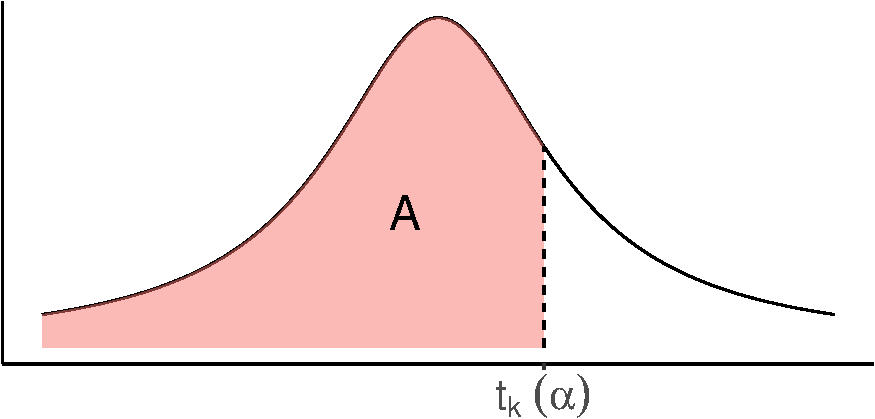
\includegraphics[width=6cm]{stat-tables_files/figure-latex/unnamed-chunk-4-1} \end{center}

\begin{table}[H]
\centering
\begin{tabular}{lrrrrrrrrrrrr}
\toprule
\multicolumn{1}{c}{ } & \multicolumn{12}{c}{$A$} \\
\cmidrule(l{3pt}r{3pt}){2-13}
$k$ & 0.60 & 0.70 & 0.80 & 0.85 & 0.90 & 0.95 & 0.975 & 0.990 & 0.9925 & 0.9950 & 0.9975 & 0.9995\\
\midrule
1 & 0.325 & 0.727 & 1.376 & 1.963 & 3.078 & 6.314 & 12.706 & 31.821 & 42.433 & 63.657 & 127.321 & 636.619\\
2 & 0.289 & 0.617 & 1.061 & 1.386 & 1.886 & 2.920 & 4.303 & 6.965 & 8.073 & 9.925 & 14.089 & 31.599\\
3 & 0.277 & 0.584 & 0.978 & 1.250 & 1.638 & 2.353 & 3.182 & 4.541 & 5.047 & 5.841 & 7.453 & 12.924\\
4 & 0.271 & 0.569 & 0.941 & 1.190 & 1.533 & 2.132 & 2.776 & 3.747 & 4.088 & 4.604 & 5.598 & 8.610\\
5 & 0.267 & 0.559 & 0.920 & 1.156 & 1.476 & 2.015 & 2.571 & 3.365 & 3.634 & 4.032 & 4.773 & 6.869\\
\addlinespace
6 & 0.265 & 0.553 & 0.906 & 1.134 & 1.440 & 1.943 & 2.447 & 3.143 & 3.372 & 3.707 & 4.317 & 5.959\\
7 & 0.263 & 0.549 & 0.896 & 1.119 & 1.415 & 1.895 & 2.365 & 2.998 & 3.203 & 3.499 & 4.029 & 5.408\\
8 & 0.262 & 0.546 & 0.889 & 1.108 & 1.397 & 1.860 & 2.306 & 2.896 & 3.085 & 3.355 & 3.833 & 5.041\\
9 & 0.261 & 0.543 & 0.883 & 1.100 & 1.383 & 1.833 & 2.262 & 2.821 & 2.998 & 3.250 & 3.690 & 4.781\\
10 & 0.260 & 0.542 & 0.879 & 1.093 & 1.372 & 1.812 & 2.228 & 2.764 & 2.932 & 3.169 & 3.581 & 4.587\\
\addlinespace
11 & 0.260 & 0.540 & 0.876 & 1.088 & 1.363 & 1.796 & 2.201 & 2.718 & 2.879 & 3.106 & 3.497 & 4.437\\
12 & 0.259 & 0.539 & 0.873 & 1.083 & 1.356 & 1.782 & 2.179 & 2.681 & 2.836 & 3.055 & 3.428 & 4.318\\
13 & 0.259 & 0.538 & 0.870 & 1.079 & 1.350 & 1.771 & 2.160 & 2.650 & 2.801 & 3.012 & 3.372 & 4.221\\
14 & 0.258 & 0.537 & 0.868 & 1.076 & 1.345 & 1.761 & 2.145 & 2.624 & 2.771 & 2.977 & 3.326 & 4.140\\
15 & 0.258 & 0.536 & 0.866 & 1.074 & 1.341 & 1.753 & 2.131 & 2.602 & 2.746 & 2.947 & 3.286 & 4.073\\
\addlinespace
16 & 0.258 & 0.535 & 0.865 & 1.071 & 1.337 & 1.746 & 2.120 & 2.583 & 2.724 & 2.921 & 3.252 & 4.015\\
17 & 0.257 & 0.534 & 0.863 & 1.069 & 1.333 & 1.740 & 2.110 & 2.567 & 2.706 & 2.898 & 3.222 & 3.965\\
18 & 0.257 & 0.534 & 0.862 & 1.067 & 1.330 & 1.734 & 2.101 & 2.552 & 2.689 & 2.878 & 3.197 & 3.922\\
19 & 0.257 & 0.533 & 0.861 & 1.066 & 1.328 & 1.729 & 2.093 & 2.539 & 2.674 & 2.861 & 3.174 & 3.883\\
20 & 0.257 & 0.533 & 0.860 & 1.064 & 1.325 & 1.725 & 2.086 & 2.528 & 2.661 & 2.845 & 3.153 & 3.850\\
\addlinespace
21 & 0.257 & 0.532 & 0.859 & 1.063 & 1.323 & 1.721 & 2.080 & 2.518 & 2.649 & 2.831 & 3.135 & 3.819\\
22 & 0.256 & 0.532 & 0.858 & 1.061 & 1.321 & 1.717 & 2.074 & 2.508 & 2.639 & 2.819 & 3.119 & 3.792\\
23 & 0.256 & 0.532 & 0.858 & 1.060 & 1.319 & 1.714 & 2.069 & 2.500 & 2.629 & 2.807 & 3.104 & 3.768\\
24 & 0.256 & 0.531 & 0.857 & 1.059 & 1.318 & 1.711 & 2.064 & 2.492 & 2.620 & 2.797 & 3.091 & 3.745\\
25 & 0.256 & 0.531 & 0.856 & 1.058 & 1.316 & 1.708 & 2.060 & 2.485 & 2.612 & 2.787 & 3.078 & 3.725\\
\addlinespace
26 & 0.256 & 0.531 & 0.856 & 1.058 & 1.315 & 1.706 & 2.056 & 2.479 & 2.605 & 2.779 & 3.067 & 3.707\\
27 & 0.256 & 0.531 & 0.855 & 1.057 & 1.314 & 1.703 & 2.052 & 2.473 & 2.598 & 2.771 & 3.057 & 3.690\\
28 & 0.256 & 0.530 & 0.855 & 1.056 & 1.313 & 1.701 & 2.048 & 2.467 & 2.592 & 2.763 & 3.047 & 3.674\\
29 & 0.256 & 0.530 & 0.854 & 1.055 & 1.311 & 1.699 & 2.045 & 2.462 & 2.586 & 2.756 & 3.038 & 3.659\\
30 & 0.256 & 0.530 & 0.854 & 1.055 & 1.310 & 1.697 & 2.042 & 2.457 & 2.581 & 2.750 & 3.030 & 3.646\\
\addlinespace
40 & 0.255 & 0.529 & 0.851 & 1.050 & 1.303 & 1.684 & 2.021 & 2.423 & 2.542 & 2.704 & 2.971 & 3.551\\
60 & 0.254 & 0.527 & 0.848 & 1.045 & 1.296 & 1.671 & 2.000 & 2.390 & 2.504 & 2.660 & 2.915 & 3.460\\
120 & 0.254 & 0.526 & 0.845 & 1.041 & 1.289 & 1.658 & 1.980 & 2.358 & 2.468 & 2.617 & 2.860 & 3.373\\
$\infty$ & 0.253 & 0.524 & 0.842 & 1.036 & 1.282 & 1.645 & 1.960 & 2.326 & 2.432 & 2.576 & 2.807 & 3.291\\
\bottomrule
\end{tabular}
\end{table}

\hypertarget{table-3.1-percentiles-of-the-f-distribution.}{%
\subsubsection{\texorpdfstring{Table 3.1: Percentiles of the
\(F\)-distribution.}{Table 3.1: Percentiles of the F-distribution.}}\label{table-3.1-percentiles-of-the-f-distribution.}}

\vspace{-0.4em}

Each table entry is
\(F_{k_1,k_2}(\alpha) = F_{k_2,k_1}^{-1}(1-\alpha)\), where
\(\text{P}\big(X < F_{k_1,k_2}(\alpha)\big)=A=1-\alpha\) with
\(X\sim F_{k_1,k_2}\).

\begin{center}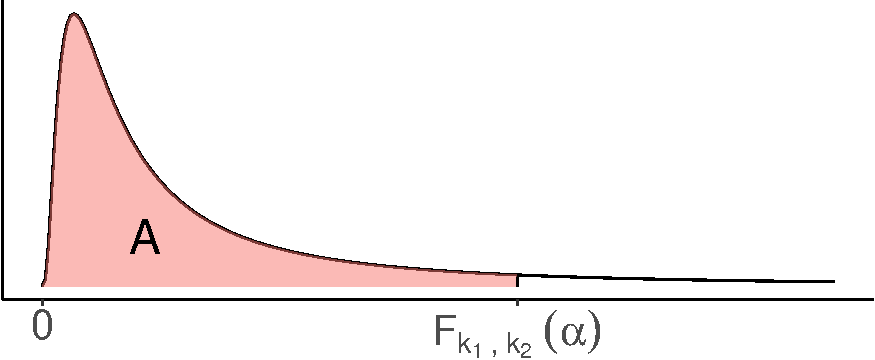
\includegraphics[width=6cm]{stat-tables_files/figure-latex/unnamed-chunk-5-1} \end{center}
\vspace{-0.6em}
\begin{table}[H]
\centering
\begin{tabular}{lrrrrrrrrrr}
\toprule
\multicolumn{1}{c}{ } & \multicolumn{10}{c}{$k_1$} \\
\cmidrule(l{3pt}r{3pt}){2-11}
\hspace{1.1em}$A$ & 1 & 2 & 3 & 4 & 5 & 6 & 7 & 8 & 9 & 10\\
\midrule
\addlinespace[0.3em]
\multicolumn{11}{l}{\textbf{$k_2=1$}}\\
\hspace{1em}0.5 & 1.00 & 1.50 & 1.71 & 1.82 & 1.89 & 1.94 & 1.98 & 2.00 & 2.03 & 2.04\\
\hspace{1em}0.9 & 39.9 & 49.5 & 53.6 & 55.8 & 57.2 & 58.2 & 58.9 & 59.4 & 59.9 & 60.2\\
\hspace{1em}0.95 & 161 & 199 & 216 & 225 & 230 & 234 & 237 & 239 & 241 & 242\\
\hspace{1em}0.975 & 648 & 799 & 864 & 900 & 922 & 937 & 948 & 957 & 963 & 969\\
\hspace{1em}0.99 & 4052 & 4999 & 5403 & 5625 & 5764 & 5859 & 5928 & 5981 & 6022 & 6056\\
\hspace{1em}0.995 & 16211 & 19999 & 21615 & 22500 & 23056 & 23437 & 23715 & 23925 & 24091 & 24224\\
\hspace{1em}0.999 & 405284 & 499999 & 540379 & 562500 & 576405 & 585937 & 592873 & 598144 & 602284 & 605621\\
\addlinespace[0.3em]
\multicolumn{11}{l}{\textbf{$k_2=2$}}\\
\hspace{1em}0.5 & 0.67 & 1.00 & 1.13 & 1.21 & 1.25 & 1.28 & 1.30 & 1.32 & 1.33 & 1.35\\
\hspace{1em}0.9 & 8.53 & 9.00 & 9.16 & 9.24 & 9.29 & 9.33 & 9.35 & 9.37 & 9.38 & 9.39\\
\hspace{1em}0.95 & 18.5 & 19.0 & 19.2 & 19.2 & 19.3 & 19.3 & 19.4 & 19.4 & 19.4 & 19.4\\
\hspace{1em}0.975 & 38.5 & 39.0 & 39.2 & 39.2 & 39.3 & 39.3 & 39.4 & 39.4 & 39.4 & 39.4\\
\hspace{1em}0.99 & 98.5 & 99.0 & 99.2 & 99.2 & 99.3 & 99.3 & 99.4 & 99.4 & 99.4 & 99.4\\
\hspace{1em}0.995 & 198.5 & 199.0 & 199.2 & 199.2 & 199.3 & 199.3 & 199.4 & 199.4 & 199.4 & 199.4\\
\hspace{1em}0.999 & 998.5 & 999.0 & 999.2 & 999.2 & 999.3 & 999.3 & 999.4 & 999.4 & 999.4 & 999.4\\
\addlinespace[0.3em]
\multicolumn{11}{l}{\textbf{$k_2=3$}}\\
\hspace{1em}0.5 & 0.59 & 0.88 & 1.00 & 1.06 & 1.10 & 1.13 & 1.15 & 1.16 & 1.17 & 1.18\\
\hspace{1em}0.9 & 5.54 & 5.46 & 5.39 & 5.34 & 5.31 & 5.28 & 5.27 & 5.25 & 5.24 & 5.23\\
\hspace{1em}0.95 & 10.13 & 9.55 & 9.28 & 9.12 & 9.01 & 8.94 & 8.89 & 8.85 & 8.81 & 8.79\\
\hspace{1em}0.975 & 17.4 & 16.0 & 15.4 & 15.1 & 14.9 & 14.7 & 14.6 & 14.5 & 14.5 & 14.4\\
\hspace{1em}0.99 & 34.1 & 30.8 & 29.5 & 28.7 & 28.2 & 27.9 & 27.7 & 27.5 & 27.3 & 27.2\\
\hspace{1em}0.995 & 55.6 & 49.8 & 47.5 & 46.2 & 45.4 & 44.8 & 44.4 & 44.1 & 43.9 & 43.7\\
\hspace{1em}0.999 & 167.0 & 148.5 & 141.1 & 137.1 & 134.6 & 132.8 & 131.6 & 130.6 & 129.9 & 129.2\\
\addlinespace[0.3em]
\multicolumn{11}{l}{\textbf{$k_2=4$}}\\
\hspace{1em}0.5 & 0.55 & 0.83 & 0.94 & 1.00 & 1.04 & 1.06 & 1.08 & 1.09 & 1.10 & 1.11\\
\hspace{1em}0.9 & 4.54 & 4.32 & 4.19 & 4.11 & 4.05 & 4.01 & 3.98 & 3.95 & 3.94 & 3.92\\
\hspace{1em}0.95 & 7.7 & 6.9 & 6.6 & 6.4 & 6.3 & 6.2 & 6.1 & 6.0 & 6.0 & 6.0\\
\hspace{1em}0.975 & 12.2 & 10.6 & 10.0 & 9.6 & 9.4 & 9.2 & 9.1 & 9.0 & 8.9 & 8.8\\
\hspace{1em}0.99 & 21.2 & 18.0 & 16.7 & 16.0 & 15.5 & 15.2 & 15.0 & 14.8 & 14.7 & 14.5\\
\hspace{1em}0.995 & 31.3 & 26.3 & 24.3 & 23.2 & 22.5 & 22.0 & 21.6 & 21.4 & 21.1 & 21.0\\
\hspace{1em}0.999 & 74.1 & 61.2 & 56.2 & 53.4 & 51.7 & 50.5 & 49.7 & 49.0 & 48.5 & 48.1\\
\addlinespace[0.3em]
\multicolumn{11}{l}{\textbf{$k_2=5$}}\\
\hspace{1em}0.5 & 0.53 & 0.80 & 0.91 & 0.96 & 1.00 & 1.02 & 1.04 & 1.05 & 1.06 & 1.07\\
\hspace{1em}0.9 & 4.06 & 3.78 & 3.62 & 3.52 & 3.45 & 3.40 & 3.37 & 3.34 & 3.32 & 3.30\\
\hspace{1em}0.95 & 6.6 & 5.8 & 5.4 & 5.2 & 5.1 & 5.0 & 4.9 & 4.8 & 4.8 & 4.7\\
\hspace{1em}0.975 & 10.0 & 8.4 & 7.8 & 7.4 & 7.1 & 7.0 & 6.9 & 6.8 & 6.7 & 6.6\\
\hspace{1em}0.99 & 16.3 & 13.3 & 12.1 & 11.4 & 11.0 & 10.7 & 10.5 & 10.3 & 10.2 & 10.1\\
\hspace{1em}0.995 & 22.8 & 18.3 & 16.5 & 15.6 & 14.9 & 14.5 & 14.2 & 14.0 & 13.8 & 13.6\\
\hspace{1em}0.999 & 47.2 & 37.1 & 33.2 & 31.1 & 29.8 & 28.8 & 28.2 & 27.6 & 27.2 & 26.9\\
\bottomrule
\end{tabular}
\end{table}

\hypertarget{table-3.2-continued-percentiles-of-the-f-distribution.}{%
\subsubsection{\texorpdfstring{Table 3.2: (Continued) Percentiles of the
\(F\)-distribution.}{Table 3.2: (Continued) Percentiles of the F-distribution.}}\label{table-3.2-continued-percentiles-of-the-f-distribution.}}

\begin{table}[H]
\centering
\begin{tabular}{lrrrrrrrrrr}
\toprule
\multicolumn{1}{c}{ } & \multicolumn{10}{c}{$k_1$} \\
\cmidrule(l{3pt}r{3pt}){2-11}
\hspace{1.1em}$A$ & 11 & 12 & 13 & 14 & 15 & 20 & 30 & 60 & 120 & $\infty$\\
\midrule
\addlinespace[0.3em]
\multicolumn{11}{l}{\textbf{$k_2=1$}}\\
\hspace{1em}0.5 & 2.06 & 2.07 & 2.08 & 2.09 & 2.09 & 2.12 & 2.15 & 2.17 & 2.18 & 2.20\\
\hspace{1em}0.9 & 60.5 & 60.7 & 60.9 & 61.1 & 61.2 & 61.7 & 62.3 & 62.8 & 63.1 & 63.3\\
\hspace{1em}0.95 & 243 & 244 & 245 & 245 & 246 & 248 & 250 & 252 & 253 & 254\\
\hspace{1em}0.975 & 973 & 977 & 980 & 983 & 985 & 993 & 1001 & 1010 & 1014 & 1018\\
\hspace{1em}0.99 & 6083 & 6106 & 6126 & 6143 & 6157 & 6209 & 6261 & 6313 & 6339 & 6366\\
\hspace{1em}0.995 & 24334 & 24426 & 24505 & 24572 & 24630 & 24836 & 25044 & 25253 & 25359 & 25464\\
\hspace{1em}0.999 & 608368 & 610668 & 612622 & 614303 & 615764 & 620908 & 626099 & 631337 & 633972 & 636619\\
\addlinespace[0.3em]
\multicolumn{11}{l}{\textbf{$k_2=2$}}\\
\hspace{1em}0.5 & 1.35 & 1.36 & 1.37 & 1.37 & 1.38 & 1.39 & 1.41 & 1.43 & 1.43 & 1.44\\
\hspace{1em}0.9 & 9.40 & 9.41 & 9.41 & 9.42 & 9.42 & 9.44 & 9.46 & 9.47 & 9.48 & 9.49\\
\hspace{1em}0.95 & 19.4 & 19.4 & 19.4 & 19.4 & 19.4 & 19.4 & 19.5 & 19.5 & 19.5 & 19.5\\
\hspace{1em}0.975 & 39.4 & 39.4 & 39.4 & 39.4 & 39.4 & 39.4 & 39.5 & 39.5 & 39.5 & 39.5\\
\hspace{1em}0.99 & 99.4 & 99.4 & 99.4 & 99.4 & 99.4 & 99.4 & 99.5 & 99.5 & 99.5 & 99.5\\
\hspace{1em}0.995 & 199.4 & 199.4 & 199.4 & 199.4 & 199.4 & 199.4 & 199.5 & 199.5 & 199.5 & 199.5\\
\hspace{1em}0.999 & 999.4 & 999.4 & 999.4 & 999.4 & 999.4 & 999.4 & 999.5 & 999.5 & 999.5 & 999.5\\
\addlinespace[0.3em]
\multicolumn{11}{l}{\textbf{$k_2=3$}}\\
\hspace{1em}0.5 & 1.19 & 1.20 & 1.20 & 1.21 & 1.21 & 1.23 & 1.24 & 1.25 & 1.26 & 1.27\\
\hspace{1em}0.9 & 5.22 & 5.22 & 5.21 & 5.20 & 5.20 & 5.18 & 5.17 & 5.15 & 5.14 & 5.13\\
\hspace{1em}0.95 & 8.76 & 8.74 & 8.73 & 8.71 & 8.70 & 8.66 & 8.62 & 8.57 & 8.55 & 8.53\\
\hspace{1em}0.975 & 14.4 & 14.3 & 14.3 & 14.3 & 14.3 & 14.2 & 14.1 & 14.0 & 13.9 & 13.9\\
\hspace{1em}0.99 & 27.1 & 27.1 & 27.0 & 26.9 & 26.9 & 26.7 & 26.5 & 26.3 & 26.2 & 26.1\\
\hspace{1em}0.995 & 43.5 & 43.4 & 43.3 & 43.2 & 43.1 & 42.8 & 42.5 & 42.1 & 42.0 & 41.8\\
\hspace{1em}0.999 & 128.7 & 128.3 & 128.0 & 127.6 & 127.4 & 126.4 & 125.4 & 124.5 & 124.0 & 123.5\\
\addlinespace[0.3em]
\multicolumn{11}{l}{\textbf{$k_2=4$}}\\
\hspace{1em}0.5 & 1.12 & 1.13 & 1.13 & 1.13 & 1.14 & 1.15 & 1.16 & 1.18 & 1.18 & 1.19\\
\hspace{1em}0.9 & 3.91 & 3.90 & 3.89 & 3.88 & 3.87 & 3.84 & 3.82 & 3.79 & 3.78 & 3.76\\
\hspace{1em}0.95 & 5.9 & 5.9 & 5.9 & 5.9 & 5.9 & 5.8 & 5.7 & 5.7 & 5.7 & 5.6\\
\hspace{1em}0.975 & 8.8 & 8.8 & 8.7 & 8.7 & 8.7 & 8.6 & 8.5 & 8.4 & 8.3 & 8.3\\
\hspace{1em}0.99 & 14.5 & 14.4 & 14.3 & 14.2 & 14.2 & 14.0 & 13.8 & 13.7 & 13.6 & 13.5\\
\hspace{1em}0.995 & 20.8 & 20.7 & 20.6 & 20.5 & 20.4 & 20.2 & 19.9 & 19.6 & 19.5 & 19.3\\
\hspace{1em}0.999 & 47.7 & 47.4 & 47.2 & 46.9 & 46.8 & 46.1 & 45.4 & 44.7 & 44.4 & 44.1\\
\addlinespace[0.3em]
\multicolumn{11}{l}{\textbf{$k_2=5$}}\\
\hspace{1em}0.5 & 1.08 & 1.09 & 1.09 & 1.09 & 1.10 & 1.11 & 1.12 & 1.14 & 1.14 & 1.15\\
\hspace{1em}0.9 & 3.28 & 3.27 & 3.26 & 3.25 & 3.24 & 3.21 & 3.17 & 3.14 & 3.12 & 3.10\\
\hspace{1em}0.95 & 4.7 & 4.7 & 4.7 & 4.6 & 4.6 & 4.6 & 4.5 & 4.4 & 4.4 & 4.4\\
\hspace{1em}0.975 & 6.6 & 6.5 & 6.5 & 6.5 & 6.4 & 6.3 & 6.2 & 6.1 & 6.1 & 6.0\\
\hspace{1em}0.99 & 10.0 & 9.9 & 9.8 & 9.8 & 9.7 & 9.6 & 9.4 & 9.2 & 9.1 & 9.0\\
\hspace{1em}0.995 & 13.5 & 13.4 & 13.3 & 13.2 & 13.1 & 12.9 & 12.7 & 12.4 & 12.3 & 12.1\\
\hspace{1em}0.999 & 26.6 & 26.4 & 26.2 & 26.1 & 25.9 & 25.4 & 24.9 & 24.3 & 24.1 & 23.8\\
\bottomrule
\end{tabular}
\end{table}

\hypertarget{table-3.3-continued-percentiles-of-the-f-distribution.}{%
\subsubsection{\texorpdfstring{Table 3.3: (Continued) Percentiles of the
\(F\)-distribution.}{Table 3.3: (Continued) Percentiles of the F-distribution.}}\label{table-3.3-continued-percentiles-of-the-f-distribution.}}

\begin{table}[H]
\centering
\begin{tabular}{lrrrrrrrrrr}
\toprule
\multicolumn{1}{c}{ } & \multicolumn{10}{c}{$k_1$} \\
\cmidrule(l{3pt}r{3pt}){2-11}
\hspace{1.1em}$A$ & 1 & 2 & 3 & 4 & 5 & 6 & 7 & 8 & 9 & 10\\
\midrule
\addlinespace[0.3em]
\multicolumn{11}{l}{\textbf{$k_2=6$}}\\
\hspace{1em}0.5 & 0.515 & 0.780 & 0.886 & 0.942 & 0.977 & 1.000 & 1.017 & 1.030 & 1.040 & 1.048\\
\hspace{1em}0.9 & 3.78 & 3.46 & 3.29 & 3.18 & 3.11 & 3.05 & 3.01 & 2.98 & 2.96 & 2.94\\
\hspace{1em}0.95 & 5.99 & 5.14 & 4.76 & 4.53 & 4.39 & 4.28 & 4.21 & 4.15 & 4.10 & 4.06\\
\hspace{1em}0.975 & 8.81 & 7.26 & 6.60 & 6.23 & 5.99 & 5.82 & 5.70 & 5.60 & 5.52 & 5.46\\
\hspace{1em}0.99 & 13.75 & 10.92 & 9.78 & 9.15 & 8.75 & 8.47 & 8.26 & 8.10 & 7.98 & 7.87\\
\hspace{1em}0.995 & 18.63 & 14.54 & 12.92 & 12.03 & 11.46 & 11.07 & 10.79 & 10.57 & 10.39 & 10.25\\
\hspace{1em}0.999 & 35.51 & 27.00 & 23.70 & 21.92 & 20.80 & 20.03 & 19.46 & 19.03 & 18.69 & 18.41\\
\addlinespace[0.3em]
\multicolumn{11}{l}{\textbf{$k_2=7$}}\\
\hspace{1em}0.5 & 0.506 & 0.767 & 0.871 & 0.926 & 0.960 & 0.983 & 1.000 & 1.013 & 1.022 & 1.030\\
\hspace{1em}0.9 & 3.59 & 3.26 & 3.07 & 2.96 & 2.88 & 2.83 & 2.78 & 2.75 & 2.72 & 2.70\\
\hspace{1em}0.95 & 5.59 & 4.74 & 4.35 & 4.12 & 3.97 & 3.87 & 3.79 & 3.73 & 3.68 & 3.64\\
\hspace{1em}0.975 & 8.07 & 6.54 & 5.89 & 5.52 & 5.29 & 5.12 & 4.99 & 4.90 & 4.82 & 4.76\\
\hspace{1em}0.99 & 12.25 & 9.55 & 8.45 & 7.85 & 7.46 & 7.19 & 6.99 & 6.84 & 6.72 & 6.62\\
\hspace{1em}0.995 & 16.24 & 12.40 & 10.88 & 10.05 & 9.52 & 9.16 & 8.89 & 8.68 & 8.51 & 8.38\\
\hspace{1em}0.999 & 29.25 & 21.69 & 18.77 & 17.20 & 16.21 & 15.52 & 15.02 & 14.63 & 14.33 & 14.08\\
\addlinespace[0.3em]
\multicolumn{11}{l}{\textbf{$k_2=8$}}\\
\hspace{1em}0.5 & 0.499 & 0.757 & 0.860 & 0.915 & 0.948 & 0.971 & 0.988 & 1.000 & 1.010 & 1.018\\
\hspace{1em}0.9 & 3.46 & 3.11 & 2.92 & 2.81 & 2.73 & 2.67 & 2.62 & 2.59 & 2.56 & 2.54\\
\hspace{1em}0.95 & 5.32 & 4.46 & 4.07 & 3.84 & 3.69 & 3.58 & 3.50 & 3.44 & 3.39 & 3.35\\
\hspace{1em}0.975 & 7.57 & 6.06 & 5.42 & 5.05 & 4.82 & 4.65 & 4.53 & 4.43 & 4.36 & 4.30\\
\hspace{1em}0.99 & 11.26 & 8.65 & 7.59 & 7.01 & 6.63 & 6.37 & 6.18 & 6.03 & 5.91 & 5.81\\
\hspace{1em}0.995 & 14.69 & 11.04 & 9.60 & 8.81 & 8.30 & 7.95 & 7.69 & 7.50 & 7.34 & 7.21\\
\hspace{1em}0.999 & 25.41 & 18.49 & 15.83 & 14.39 & 13.48 & 12.86 & 12.40 & 12.05 & 11.77 & 11.54\\
\addlinespace[0.3em]
\multicolumn{11}{l}{\textbf{$k_2=9$}}\\
\hspace{1em}0.5 & 0.494 & 0.749 & 0.852 & 0.906 & 0.939 & 0.962 & 0.978 & 0.990 & 1.000 & 1.008\\
\hspace{1em}0.9 & 3.36 & 3.01 & 2.81 & 2.69 & 2.61 & 2.55 & 2.51 & 2.47 & 2.44 & 2.42\\
\hspace{1em}0.95 & 5.12 & 4.26 & 3.86 & 3.63 & 3.48 & 3.37 & 3.29 & 3.23 & 3.18 & 3.14\\
\hspace{1em}0.975 & 7.21 & 5.71 & 5.08 & 4.72 & 4.48 & 4.32 & 4.20 & 4.10 & 4.03 & 3.96\\
\hspace{1em}0.99 & 10.56 & 8.02 & 6.99 & 6.42 & 6.06 & 5.80 & 5.61 & 5.47 & 5.35 & 5.26\\
\hspace{1em}0.995 & 13.61 & 10.11 & 8.72 & 7.96 & 7.47 & 7.13 & 6.88 & 6.69 & 6.54 & 6.42\\
\hspace{1em}0.999 & 22.86 & 16.39 & 13.90 & 12.56 & 11.71 & 11.13 & 10.70 & 10.37 & 10.11 & 9.89\\
\addlinespace[0.3em]
\multicolumn{11}{l}{\textbf{$k_2=10$}}\\
\hspace{1em}0.5 & 0.490 & 0.743 & 0.845 & 0.899 & 0.932 & 0.954 & 0.971 & 0.983 & 0.992 & 1.000\\
\hspace{1em}0.9 & 3.29 & 2.92 & 2.73 & 2.61 & 2.52 & 2.46 & 2.41 & 2.38 & 2.35 & 2.32\\
\hspace{1em}0.95 & 4.96 & 4.10 & 3.71 & 3.48 & 3.33 & 3.22 & 3.14 & 3.07 & 3.02 & 2.98\\
\hspace{1em}0.975 & 6.94 & 5.46 & 4.83 & 4.47 & 4.24 & 4.07 & 3.95 & 3.85 & 3.78 & 3.72\\
\hspace{1em}0.99 & 10.04 & 7.56 & 6.55 & 5.99 & 5.64 & 5.39 & 5.20 & 5.06 & 4.94 & 4.85\\
\hspace{1em}0.995 & 12.83 & 9.43 & 8.08 & 7.34 & 6.87 & 6.54 & 6.30 & 6.12 & 5.97 & 5.85\\
\hspace{1em}0.999 & 21.04 & 14.91 & 12.55 & 11.28 & 10.48 & 9.93 & 9.52 & 9.20 & 8.96 & 8.75\\
\bottomrule
\end{tabular}
\end{table}

\hypertarget{table-3.4-continued-percentiles-of-the-f-distribution.}{%
\subsubsection{\texorpdfstring{Table 3.4: (Continued) Percentiles of the
\(F\)-distribution.}{Table 3.4: (Continued) Percentiles of the F-distribution.}}\label{table-3.4-continued-percentiles-of-the-f-distribution.}}

\begin{table}[H]
\centering
\begin{tabular}{lrrrrrrrrrr}
\toprule
\multicolumn{1}{c}{ } & \multicolumn{10}{c}{$k_1$} \\
\cmidrule(l{3pt}r{3pt}){2-11}
\hspace{1.1em}$A$ & 11 & 12 & 13 & 14 & 15 & 20 & 30 & 60 & 120 & $\infty$\\
\midrule
\addlinespace[0.3em]
\multicolumn{11}{l}{\textbf{$k_2=6$}}\\
\hspace{1em}0.5 & 1.054 & 1.060 & 1.065 & 1.069 & 1.072 & 1.084 & 1.097 & 1.109 & 1.116 & 1.122\\
\hspace{1em}0.9 & 2.920 & 2.905 & 2.892 & 2.881 & 2.871 & 2.836 & 2.800 & 2.762 & 2.742 & 2.722\\
\hspace{1em}0.95 & 4.03 & 4.00 & 3.98 & 3.96 & 3.94 & 3.87 & 3.81 & 3.74 & 3.70 & 3.67\\
\hspace{1em}0.975 & 5.41 & 5.37 & 5.33 & 5.30 & 5.27 & 5.17 & 5.07 & 4.96 & 4.90 & 4.85\\
\hspace{1em}0.99 & 7.79 & 7.72 & 7.66 & 7.60 & 7.56 & 7.40 & 7.23 & 7.06 & 6.97 & 6.88\\
\hspace{1em}0.995 & 10.13 & 10.03 & 9.95 & 9.88 & 9.81 & 9.59 & 9.36 & 9.12 & 9.00 & 8.88\\
\hspace{1em}0.999 & 18.18 & 17.99 & 17.82 & 17.68 & 17.56 & 17.12 & 16.67 & 16.21 & 15.98 & 15.75\\
\addlinespace[0.3em]
\multicolumn{11}{l}{\textbf{$k_2=7$}}\\
\hspace{1em}0.5 & 1.037 & 1.042 & 1.047 & 1.051 & 1.054 & 1.066 & 1.079 & 1.091 & 1.097 & 1.103\\
\hspace{1em}0.9 & 2.684 & 2.668 & 2.654 & 2.643 & 2.632 & 2.595 & 2.555 & 2.514 & 2.493 & 2.471\\
\hspace{1em}0.95 & 3.60 & 3.57 & 3.55 & 3.53 & 3.51 & 3.44 & 3.38 & 3.30 & 3.27 & 3.23\\
\hspace{1em}0.975 & 4.71 & 4.67 & 4.63 & 4.60 & 4.57 & 4.47 & 4.36 & 4.25 & 4.20 & 4.14\\
\hspace{1em}0.99 & 6.54 & 6.47 & 6.41 & 6.36 & 6.31 & 6.16 & 5.99 & 5.82 & 5.74 & 5.65\\
\hspace{1em}0.995 & 8.27 & 8.18 & 8.10 & 8.03 & 7.97 & 7.75 & 7.53 & 7.31 & 7.19 & 7.08\\
\hspace{1em}0.999 & 13.88 & 13.71 & 13.56 & 13.43 & 13.32 & 12.93 & 12.53 & 12.12 & 11.91 & 11.70\\
\addlinespace[0.3em]
\multicolumn{11}{l}{\textbf{$k_2=8$}}\\
\hspace{1em}0.5 & 1.024 & 1.029 & 1.034 & 1.038 & 1.041 & 1.053 & 1.065 & 1.077 & 1.083 & 1.089\\
\hspace{1em}0.9 & 2.52 & 2.50 & 2.49 & 2.48 & 2.46 & 2.42 & 2.38 & 2.34 & 2.32 & 2.29\\
\hspace{1em}0.95 & 3.31 & 3.28 & 3.26 & 3.24 & 3.22 & 3.15 & 3.08 & 3.01 & 2.97 & 2.93\\
\hspace{1em}0.975 & 4.24 & 4.20 & 4.16 & 4.13 & 4.10 & 4.00 & 3.89 & 3.78 & 3.73 & 3.67\\
\hspace{1em}0.99 & 5.73 & 5.67 & 5.61 & 5.56 & 5.52 & 5.36 & 5.20 & 5.03 & 4.95 & 4.86\\
\hspace{1em}0.995 & 7.10 & 7.01 & 6.94 & 6.87 & 6.81 & 6.61 & 6.40 & 6.18 & 6.06 & 5.95\\
\hspace{1em}0.999 & 11.35 & 11.19 & 11.06 & 10.94 & 10.84 & 10.48 & 10.11 & 9.73 & 9.53 & 9.33\\
\addlinespace[0.3em]
\multicolumn{11}{l}{\textbf{$k_2=9$}}\\
\hspace{1em}0.5 & 1.014 & 1.019 & 1.024 & 1.028 & 1.031 & 1.043 & 1.055 & 1.067 & 1.073 & 1.079\\
\hspace{1em}0.9 & 2.40 & 2.38 & 2.36 & 2.35 & 2.34 & 2.30 & 2.25 & 2.21 & 2.18 & 2.16\\
\hspace{1em}0.95 & 3.10 & 3.07 & 3.05 & 3.03 & 3.01 & 2.94 & 2.86 & 2.79 & 2.75 & 2.71\\
\hspace{1em}0.975 & 3.91 & 3.87 & 3.83 & 3.80 & 3.77 & 3.67 & 3.56 & 3.45 & 3.39 & 3.33\\
\hspace{1em}0.99 & 5.18 & 5.11 & 5.05 & 5.01 & 4.96 & 4.81 & 4.65 & 4.48 & 4.40 & 4.31\\
\hspace{1em}0.995 & 6.31 & 6.23 & 6.15 & 6.09 & 6.03 & 5.83 & 5.62 & 5.41 & 5.30 & 5.19\\
\hspace{1em}0.999 & 9.72 & 9.57 & 9.44 & 9.33 & 9.24 & 8.90 & 8.55 & 8.19 & 8.00 & 7.81\\
\addlinespace[0.3em]
\multicolumn{11}{l}{\textbf{$k_2=10$}}\\
\hspace{1em}0.5 & 1.006 & 1.012 & 1.016 & 1.020 & 1.023 & 1.035 & 1.047 & 1.059 & 1.064 & 1.070\\
\hspace{1em}0.9 & 2.30 & 2.28 & 2.27 & 2.26 & 2.24 & 2.20 & 2.16 & 2.11 & 2.08 & 2.06\\
\hspace{1em}0.95 & 2.94 & 2.91 & 2.89 & 2.86 & 2.85 & 2.77 & 2.70 & 2.62 & 2.58 & 2.54\\
\hspace{1em}0.975 & 3.66 & 3.62 & 3.58 & 3.55 & 3.52 & 3.42 & 3.31 & 3.20 & 3.14 & 3.08\\
\hspace{1em}0.99 & 4.77 & 4.71 & 4.65 & 4.60 & 4.56 & 4.41 & 4.25 & 4.08 & 4.00 & 3.91\\
\hspace{1em}0.995 & 5.75 & 5.66 & 5.59 & 5.53 & 5.47 & 5.27 & 5.07 & 4.86 & 4.75 & 4.64\\
\hspace{1em}0.999 & 8.59 & 8.45 & 8.32 & 8.22 & 8.13 & 7.80 & 7.47 & 7.12 & 6.94 & 6.76\\
\bottomrule
\end{tabular}
\end{table}

\hypertarget{table-3.5-continued-percentiles-of-the-f-distribution.}{%
\subsubsection{\texorpdfstring{Table 3.5: (Continued) Percentiles of the
\(F\)-distribution.}{Table 3.5: (Continued) Percentiles of the F-distribution.}}\label{table-3.5-continued-percentiles-of-the-f-distribution.}}

\begin{table}[H]
\centering
\begin{tabular}{lrrrrrrrrrr}
\toprule
\multicolumn{1}{c}{ } & \multicolumn{10}{c}{$k_1$} \\
\cmidrule(l{3pt}r{3pt}){2-11}
\hspace{1.1em}$A$ & 1 & 2 & 3 & 4 & 5 & 6 & 7 & 8 & 9 & 10\\
\midrule
\addlinespace[0.3em]
\multicolumn{11}{l}{\textbf{$k_2=11$}}\\
\hspace{1em}0.5 & 0.486 & 0.739 & 0.840 & 0.893 & 0.926 & 0.948 & 0.964 & 0.977 & 0.986 & 0.994\\
\hspace{1em}0.9 & 3.23 & 2.86 & 2.66 & 2.54 & 2.45 & 2.39 & 2.34 & 2.30 & 2.27 & 2.25\\
\hspace{1em}0.95 & 4.84 & 3.98 & 3.59 & 3.36 & 3.20 & 3.09 & 3.01 & 2.95 & 2.90 & 2.85\\
\hspace{1em}0.975 & 6.72 & 5.26 & 4.63 & 4.28 & 4.04 & 3.88 & 3.76 & 3.66 & 3.59 & 3.53\\
\hspace{1em}0.99 & 9.65 & 7.21 & 6.22 & 5.67 & 5.32 & 5.07 & 4.89 & 4.74 & 4.63 & 4.54\\
\hspace{1em}0.995 & 12.23 & 8.91 & 7.60 & 6.88 & 6.42 & 6.10 & 5.86 & 5.68 & 5.54 & 5.42\\
\hspace{1em}0.999 & 19.69 & 13.81 & 11.56 & 10.35 & 9.58 & 9.05 & 8.66 & 8.35 & 8.12 & 7.92\\
\addlinespace[0.3em]
\multicolumn{11}{l}{\textbf{$k_2=12$}}\\
\hspace{1em}0.5 & 0.484 & 0.735 & 0.835 & 0.888 & 0.921 & 0.943 & 0.959 & 0.972 & 0.981 & 0.989\\
\hspace{1em}0.9 & 3.18 & 2.81 & 2.61 & 2.48 & 2.39 & 2.33 & 2.28 & 2.24 & 2.21 & 2.19\\
\hspace{1em}0.95 & 4.75 & 3.89 & 3.49 & 3.26 & 3.11 & 3.00 & 2.91 & 2.85 & 2.80 & 2.75\\
\hspace{1em}0.975 & 6.55 & 5.10 & 4.47 & 4.12 & 3.89 & 3.73 & 3.61 & 3.51 & 3.44 & 3.37\\
\hspace{1em}0.99 & 9.33 & 6.93 & 5.95 & 5.41 & 5.06 & 4.82 & 4.64 & 4.50 & 4.39 & 4.30\\
\hspace{1em}0.995 & 11.75 & 8.51 & 7.23 & 6.52 & 6.07 & 5.76 & 5.52 & 5.35 & 5.20 & 5.09\\
\hspace{1em}0.999 & 18.64 & 12.97 & 10.80 & 9.63 & 8.89 & 8.38 & 8.00 & 7.71 & 7.48 & 7.29\\
\addlinespace[0.3em]
\multicolumn{11}{l}{\textbf{$k_2=13$}}\\
\hspace{1em}0.5 & 0.481 & 0.731 & 0.832 & 0.885 & 0.917 & 0.939 & 0.955 & 0.967 & 0.977 & 0.984\\
\hspace{1em}0.9 & 3.14 & 2.76 & 2.56 & 2.43 & 2.35 & 2.28 & 2.23 & 2.20 & 2.16 & 2.14\\
\hspace{1em}0.95 & 4.67 & 3.81 & 3.41 & 3.18 & 3.03 & 2.92 & 2.83 & 2.77 & 2.71 & 2.67\\
\hspace{1em}0.975 & 6.41 & 4.97 & 4.35 & 4.00 & 3.77 & 3.60 & 3.48 & 3.39 & 3.31 & 3.25\\
\hspace{1em}0.99 & 9.07 & 6.70 & 5.74 & 5.21 & 4.86 & 4.62 & 4.44 & 4.30 & 4.19 & 4.10\\
\hspace{1em}0.995 & 11.37 & 8.19 & 6.93 & 6.23 & 5.79 & 5.48 & 5.25 & 5.08 & 4.94 & 4.82\\
\hspace{1em}0.999 & 17.82 & 12.31 & 10.21 & 9.07 & 8.35 & 7.86 & 7.49 & 7.21 & 6.98 & 6.80\\
\addlinespace[0.3em]
\multicolumn{11}{l}{\textbf{$k_2=14$}}\\
\hspace{1em}0.5 & 0.479 & 0.729 & 0.828 & 0.881 & 0.914 & 0.936 & 0.952 & 0.964 & 0.973 & 0.981\\
\hspace{1em}0.9 & 3.10 & 2.73 & 2.52 & 2.39 & 2.31 & 2.24 & 2.19 & 2.15 & 2.12 & 2.10\\
\hspace{1em}0.95 & 4.60 & 3.74 & 3.34 & 3.11 & 2.96 & 2.85 & 2.76 & 2.70 & 2.65 & 2.60\\
\hspace{1em}0.975 & 6.30 & 4.86 & 4.24 & 3.89 & 3.66 & 3.50 & 3.38 & 3.29 & 3.21 & 3.15\\
\hspace{1em}0.99 & 8.86 & 6.51 & 5.56 & 5.04 & 4.69 & 4.46 & 4.28 & 4.14 & 4.03 & 3.94\\
\hspace{1em}0.995 & 11.06 & 7.92 & 6.68 & 6.00 & 5.56 & 5.26 & 5.03 & 4.86 & 4.72 & 4.60\\
\hspace{1em}0.999 & 17.14 & 11.78 & 9.73 & 8.62 & 7.92 & 7.44 & 7.08 & 6.80 & 6.58 & 6.40\\
\addlinespace[0.3em]
\multicolumn{11}{l}{\textbf{$k_2=15$}}\\
\hspace{1em}0.5 & 0.478 & 0.726 & 0.826 & 0.878 & 0.911 & 0.933 & 0.949 & 0.960 & 0.970 & 0.977\\
\hspace{1em}0.9 & 3.07 & 2.70 & 2.49 & 2.36 & 2.27 & 2.21 & 2.16 & 2.12 & 2.09 & 2.06\\
\hspace{1em}0.95 & 4.54 & 3.68 & 3.29 & 3.06 & 2.90 & 2.79 & 2.71 & 2.64 & 2.59 & 2.54\\
\hspace{1em}0.975 & 6.20 & 4.77 & 4.15 & 3.80 & 3.58 & 3.41 & 3.29 & 3.20 & 3.12 & 3.06\\
\hspace{1em}0.99 & 8.68 & 6.36 & 5.42 & 4.89 & 4.56 & 4.32 & 4.14 & 4.00 & 3.89 & 3.80\\
\hspace{1em}0.995 & 10.80 & 7.70 & 6.48 & 5.80 & 5.37 & 5.07 & 4.85 & 4.67 & 4.54 & 4.42\\
\hspace{1em}0.999 & 16.59 & 11.34 & 9.34 & 8.25 & 7.57 & 7.09 & 6.74 & 6.47 & 6.26 & 6.08\\
\bottomrule
\end{tabular}
\end{table}

\hypertarget{table-3.6-continued-percentiles-of-the-f-distribution.}{%
\subsubsection{\texorpdfstring{Table 3.6: (Continued) Percentiles of the
\(F\)-distribution.}{Table 3.6: (Continued) Percentiles of the F-distribution.}}\label{table-3.6-continued-percentiles-of-the-f-distribution.}}

\begin{table}[H]
\centering
\begin{tabular}{lrrrrrrrrrr}
\toprule
\multicolumn{1}{c}{ } & \multicolumn{10}{c}{$k_1$} \\
\cmidrule(l{3pt}r{3pt}){2-11}
\hspace{1.1em}$A$ & 11 & 12 & 13 & 14 & 15 & 20 & 30 & 60 & 120 & $\infty$\\
\midrule
\addlinespace[0.3em]
\multicolumn{11}{l}{\textbf{$k_2=11$}}\\
\hspace{1em}0.5 & 1.000 & 1.005 & 1.010 & 1.013 & 1.017 & 1.028 & 1.040 & 1.052 & 1.058 & 1.064\\
\hspace{1em}0.9 & 2.227 & 2.209 & 2.193 & 2.179 & 2.167 & 2.123 & 2.076 & 2.026 & 2.000 & 1.972\\
\hspace{1em}0.95 & 2.82 & 2.79 & 2.76 & 2.74 & 2.72 & 2.65 & 2.57 & 2.49 & 2.45 & 2.40\\
\hspace{1em}0.975 & 3.47 & 3.43 & 3.39 & 3.36 & 3.33 & 3.23 & 3.12 & 3.00 & 2.94 & 2.88\\
\hspace{1em}0.99 & 4.46 & 4.40 & 4.34 & 4.29 & 4.25 & 4.10 & 3.94 & 3.78 & 3.69 & 3.60\\
\hspace{1em}0.995 & 5.32 & 5.24 & 5.16 & 5.10 & 5.05 & 4.86 & 4.65 & 4.45 & 4.34 & 4.23\\
\hspace{1em}0.999 & 7.76 & 7.63 & 7.51 & 7.41 & 7.32 & 7.01 & 6.68 & 6.35 & 6.18 & 6.00\\
\addlinespace[0.3em]
\multicolumn{11}{l}{\textbf{$k_2=12$}}\\
\hspace{1em}0.5 & 0.995 & 1.000 & 1.004 & 1.008 & 1.012 & 1.023 & 1.035 & 1.046 & 1.052 & 1.058\\
\hspace{1em}0.9 & 2.166 & 2.147 & 2.131 & 2.117 & 2.105 & 2.060 & 2.011 & 1.960 & 1.932 & 1.904\\
\hspace{1em}0.95 & 2.72 & 2.69 & 2.66 & 2.64 & 2.62 & 2.54 & 2.47 & 2.38 & 2.34 & 2.30\\
\hspace{1em}0.975 & 3.32 & 3.28 & 3.24 & 3.21 & 3.18 & 3.07 & 2.96 & 2.85 & 2.79 & 2.72\\
\hspace{1em}0.99 & 4.22 & 4.16 & 4.10 & 4.05 & 4.01 & 3.86 & 3.70 & 3.54 & 3.45 & 3.36\\
\hspace{1em}0.995 & 4.99 & 4.91 & 4.84 & 4.77 & 4.72 & 4.53 & 4.33 & 4.12 & 4.01 & 3.90\\
\hspace{1em}0.999 & 7.14 & 7.00 & 6.89 & 6.79 & 6.71 & 6.40 & 6.09 & 5.76 & 5.59 & 5.42\\
\addlinespace[0.3em]
\multicolumn{11}{l}{\textbf{$k_2=13$}}\\
\hspace{1em}0.5 & 0.990 & 0.996 & 1.000 & 1.004 & 1.007 & 1.019 & 1.030 & 1.042 & 1.048 & 1.054\\
\hspace{1em}0.9 & 2.116 & 2.097 & 2.080 & 2.066 & 2.053 & 2.007 & 1.958 & 1.904 & 1.876 & 1.846\\
\hspace{1em}0.95 & 2.63 & 2.60 & 2.58 & 2.55 & 2.53 & 2.46 & 2.38 & 2.30 & 2.25 & 2.21\\
\hspace{1em}0.975 & 3.20 & 3.15 & 3.12 & 3.08 & 3.05 & 2.95 & 2.84 & 2.72 & 2.66 & 2.60\\
\hspace{1em}0.99 & 4.02 & 3.96 & 3.91 & 3.86 & 3.82 & 3.66 & 3.51 & 3.34 & 3.25 & 3.17\\
\hspace{1em}0.995 & 4.72 & 4.64 & 4.57 & 4.51 & 4.46 & 4.27 & 4.07 & 3.87 & 3.76 & 3.65\\
\hspace{1em}0.999 & 6.65 & 6.52 & 6.41 & 6.31 & 6.23 & 5.93 & 5.63 & 5.30 & 5.14 & 4.97\\
\addlinespace[0.3em]
\multicolumn{11}{l}{\textbf{$k_2=14$}}\\
\hspace{1em}0.5 & 0.987 & 0.992 & 0.996 & 1.000 & 1.003 & 1.015 & 1.026 & 1.038 & 1.044 & 1.050\\
\hspace{1em}0.9 & 2.073 & 2.054 & 2.037 & 2.022 & 2.010 & 1.962 & 1.912 & 1.857 & 1.828 & 1.797\\
\hspace{1em}0.95 & 2.57 & 2.53 & 2.51 & 2.48 & 2.46 & 2.39 & 2.31 & 2.22 & 2.18 & 2.13\\
\hspace{1em}0.975 & 3.09 & 3.05 & 3.01 & 2.98 & 2.95 & 2.84 & 2.73 & 2.61 & 2.55 & 2.49\\
\hspace{1em}0.99 & 3.86 & 3.80 & 3.75 & 3.70 & 3.66 & 3.51 & 3.35 & 3.18 & 3.09 & 3.00\\
\hspace{1em}0.995 & 4.51 & 4.43 & 4.36 & 4.30 & 4.25 & 4.06 & 3.86 & 3.66 & 3.55 & 3.44\\
\hspace{1em}0.999 & 6.26 & 6.13 & 6.02 & 5.93 & 5.85 & 5.56 & 5.25 & 4.94 & 4.77 & 4.60\\
\addlinespace[0.3em]
\multicolumn{11}{l}{\textbf{$k_2=15$}}\\
\hspace{1em}0.5 & 0.983 & 0.989 & 0.993 & 0.997 & 1.000 & 1.011 & 1.023 & 1.034 & 1.040 & 1.046\\
\hspace{1em}0.9 & 2.037 & 2.017 & 2.000 & 1.985 & 1.972 & 1.924 & 1.873 & 1.817 & 1.787 & 1.755\\
\hspace{1em}0.95 & 2.51 & 2.48 & 2.45 & 2.42 & 2.40 & 2.33 & 2.25 & 2.16 & 2.11 & 2.07\\
\hspace{1em}0.975 & 3.01 & 2.96 & 2.92 & 2.89 & 2.86 & 2.76 & 2.64 & 2.52 & 2.46 & 2.40\\
\hspace{1em}0.99 & 3.73 & 3.67 & 3.61 & 3.56 & 3.52 & 3.37 & 3.21 & 3.05 & 2.96 & 2.87\\
\hspace{1em}0.995 & 4.33 & 4.25 & 4.18 & 4.12 & 4.07 & 3.88 & 3.69 & 3.48 & 3.37 & 3.26\\
\hspace{1em}0.999 & 5.94 & 5.81 & 5.71 & 5.62 & 5.54 & 5.25 & 4.95 & 4.64 & 4.47 & 4.31\\
\bottomrule
\end{tabular}
\end{table}

\hypertarget{table-3.7-continued-percentiles-of-the-f-distribution.}{%
\subsubsection{\texorpdfstring{Table 3.7: (Continued) Percentiles of the
\(F\)-distribution.}{Table 3.7: (Continued) Percentiles of the F-distribution.}}\label{table-3.7-continued-percentiles-of-the-f-distribution.}}

\begin{table}[H]
\centering
\begin{tabular}{lrrrrrrrrrr}
\toprule
\multicolumn{1}{c}{ } & \multicolumn{10}{c}{$k_1$} \\
\cmidrule(l{3pt}r{3pt}){2-11}
\hspace{1.1em}$A$ & 1 & 2 & 3 & 4 & 5 & 6 & 7 & 8 & 9 & 10\\
\midrule
\addlinespace[0.3em]
\multicolumn{11}{l}{\textbf{$k_2=20$}}\\
\hspace{1em}0.5 & 0.472 & 0.718 & 0.816 & 0.868 & 0.900 & 0.922 & 0.938 & 0.950 & 0.959 & 0.966\\
\hspace{1em}0.9 & 2.97 & 2.59 & 2.38 & 2.25 & 2.16 & 2.09 & 2.04 & 2.00 & 1.96 & 1.94\\
\hspace{1em}0.95 & 4.35 & 3.49 & 3.10 & 2.87 & 2.71 & 2.60 & 2.51 & 2.45 & 2.39 & 2.35\\
\hspace{1em}0.975 & 5.87 & 4.46 & 3.86 & 3.51 & 3.29 & 3.13 & 3.01 & 2.91 & 2.84 & 2.77\\
\hspace{1em}0.99 & 8.10 & 5.85 & 4.94 & 4.43 & 4.10 & 3.87 & 3.70 & 3.56 & 3.46 & 3.37\\
\hspace{1em}0.995 & 9.94 & 6.99 & 5.82 & 5.17 & 4.76 & 4.47 & 4.26 & 4.09 & 3.96 & 3.85\\
\hspace{1em}0.999 & 14.82 & 9.95 & 8.10 & 7.10 & 6.46 & 6.02 & 5.69 & 5.44 & 5.24 & 5.08\\
\addlinespace[0.3em]
\multicolumn{11}{l}{\textbf{$k_2=30$}}\\
\hspace{1em}0.5 & 0.466 & 0.709 & 0.807 & 0.858 & 0.890 & 0.912 & 0.927 & 0.939 & 0.948 & 0.955\\
\hspace{1em}0.9 & 2.88 & 2.49 & 2.28 & 2.14 & 2.05 & 1.98 & 1.93 & 1.88 & 1.85 & 1.82\\
\hspace{1em}0.95 & 4.17 & 3.32 & 2.92 & 2.69 & 2.53 & 2.42 & 2.33 & 2.27 & 2.21 & 2.16\\
\hspace{1em}0.975 & 5.57 & 4.18 & 3.59 & 3.25 & 3.03 & 2.87 & 2.75 & 2.65 & 2.57 & 2.51\\
\hspace{1em}0.99 & 7.56 & 5.39 & 4.51 & 4.02 & 3.70 & 3.47 & 3.30 & 3.17 & 3.07 & 2.98\\
\hspace{1em}0.995 & 9.18 & 6.35 & 5.24 & 4.62 & 4.23 & 3.95 & 3.74 & 3.58 & 3.45 & 3.34\\
\hspace{1em}0.999 & 13.29 & 8.77 & 7.05 & 6.12 & 5.53 & 5.12 & 4.82 & 4.58 & 4.39 & 4.24\\
\addlinespace[0.3em]
\multicolumn{11}{l}{\textbf{$k_2=60$}}\\
\hspace{1em}0.5 & 0.460 & 0.701 & 0.798 & 0.849 & 0.880 & 0.901 & 0.917 & 0.928 & 0.937 & 0.945\\
\hspace{1em}0.9 & 2.79 & 2.39 & 2.18 & 2.04 & 1.95 & 1.87 & 1.82 & 1.77 & 1.74 & 1.71\\
\hspace{1em}0.95 & 4.00 & 3.15 & 2.76 & 2.53 & 2.37 & 2.25 & 2.17 & 2.10 & 2.04 & 1.99\\
\hspace{1em}0.975 & 5.29 & 3.93 & 3.34 & 3.01 & 2.79 & 2.63 & 2.51 & 2.41 & 2.33 & 2.27\\
\hspace{1em}0.99 & 7.08 & 4.98 & 4.13 & 3.65 & 3.34 & 3.12 & 2.95 & 2.82 & 2.72 & 2.63\\
\hspace{1em}0.995 & 8.49 & 5.79 & 4.73 & 4.14 & 3.76 & 3.49 & 3.29 & 3.13 & 3.01 & 2.90\\
\hspace{1em}0.999 & 11.97 & 7.77 & 6.17 & 5.31 & 4.76 & 4.37 & 4.09 & 3.86 & 3.69 & 3.54\\
\addlinespace[0.3em]
\multicolumn{11}{l}{\textbf{$k_2=120$}}\\
\hspace{1em}0.5 & 0.458 & 0.697 & 0.793 & 0.844 & 0.875 & 0.896 & 0.912 & 0.923 & 0.932 & 0.939\\
\hspace{1em}0.9 & 2.75 & 2.35 & 2.13 & 1.99 & 1.90 & 1.82 & 1.77 & 1.72 & 1.68 & 1.65\\
\hspace{1em}0.95 & 3.92 & 3.07 & 2.68 & 2.45 & 2.29 & 2.18 & 2.09 & 2.02 & 1.96 & 1.91\\
\hspace{1em}0.975 & 5.15 & 3.80 & 3.23 & 2.89 & 2.67 & 2.52 & 2.39 & 2.30 & 2.22 & 2.16\\
\hspace{1em}0.99 & 6.85 & 4.79 & 3.95 & 3.48 & 3.17 & 2.96 & 2.79 & 2.66 & 2.56 & 2.47\\
\hspace{1em}0.995 & 8.18 & 5.54 & 4.50 & 3.92 & 3.55 & 3.28 & 3.09 & 2.93 & 2.81 & 2.71\\
\hspace{1em}0.999 & 11.38 & 7.32 & 5.78 & 4.95 & 4.42 & 4.04 & 3.77 & 3.55 & 3.38 & 3.24\\
\addlinespace[0.3em]
\multicolumn{11}{l}{\textbf{$k_2=\infty$}}\\
\hspace{1em}0.5 & 0.455 & 0.693 & 0.789 & 0.839 & 0.870 & 0.891 & 0.907 & 0.918 & 0.927 & 0.934\\
\hspace{1em}0.9 & 2.71 & 2.30 & 2.08 & 1.94 & 1.85 & 1.77 & 1.72 & 1.67 & 1.63 & 1.60\\
\hspace{1em}0.95 & 3.84 & 3.00 & 2.60 & 2.37 & 2.21 & 2.10 & 2.01 & 1.94 & 1.88 & 1.83\\
\hspace{1em}0.975 & 5.02 & 3.69 & 3.12 & 2.79 & 2.57 & 2.41 & 2.29 & 2.19 & 2.11 & 2.05\\
\hspace{1em}0.99 & 6.63 & 4.61 & 3.78 & 3.32 & 3.02 & 2.80 & 2.64 & 2.51 & 2.41 & 2.32\\
\hspace{1em}0.995 & 7.88 & 5.30 & 4.28 & 3.72 & 3.35 & 3.09 & 2.90 & 2.74 & 2.62 & 2.52\\
\hspace{1em}0.999 & 10.83 & 6.91 & 5.42 & 4.62 & 4.10 & 3.74 & 3.47 & 3.27 & 3.10 & 2.96\\
\bottomrule
\end{tabular}
\end{table}

\hypertarget{table-3.8-continued-percentiles-of-the-f-distribution.}{%
\subsubsection{\texorpdfstring{Table 3.8: (Continued) Percentiles of the
\(F\)-distribution.}{Table 3.8: (Continued) Percentiles of the F-distribution.}}\label{table-3.8-continued-percentiles-of-the-f-distribution.}}

\begin{table}[H]
\centering
\begin{tabular}{lrrrrrrrrrr}
\toprule
\multicolumn{1}{c}{ } & \multicolumn{10}{c}{$k_1$} \\
\cmidrule(l{3pt}r{3pt}){2-11}
\hspace{1.1em}$A$ & 11 & 12 & 13 & 14 & 15 & 20 & 30 & 60 & 120 & $\infty$\\
\midrule
\addlinespace[0.3em]
\multicolumn{11}{l}{\textbf{$k_2=20$}}\\
\hspace{1em}0.5 & 0.972 & 0.977 & 0.982 & 0.985 & 0.989 & 1.000 & 1.011 & 1.023 & 1.029 & 1.034\\
\hspace{1em}0.9 & 1.913 & 1.892 & 1.875 & 1.859 & 1.845 & 1.794 & 1.738 & 1.677 & 1.643 & 1.607\\
\hspace{1em}0.95 & 2.31 & 2.28 & 2.25 & 2.22 & 2.20 & 2.12 & 2.04 & 1.95 & 1.90 & 1.84\\
\hspace{1em}0.975 & 2.72 & 2.68 & 2.64 & 2.60 & 2.57 & 2.46 & 2.35 & 2.22 & 2.16 & 2.09\\
\hspace{1em}0.99 & 3.29 & 3.23 & 3.18 & 3.13 & 3.09 & 2.94 & 2.78 & 2.61 & 2.52 & 2.42\\
\hspace{1em}0.995 & 3.76 & 3.68 & 3.61 & 3.55 & 3.50 & 3.32 & 3.12 & 2.92 & 2.81 & 2.69\\
\hspace{1em}0.999 & 4.94 & 4.82 & 4.72 & 4.64 & 4.56 & 4.29 & 4.00 & 3.70 & 3.54 & 3.38\\
\addlinespace[0.3em]
\multicolumn{11}{l}{\textbf{$k_2=30$}}\\
\hspace{1em}0.5 & 0.961 & 0.966 & 0.971 & 0.974 & 0.978 & 0.989 & 1.000 & 1.011 & 1.017 & 1.023\\
\hspace{1em}0.9 & 1.794 & 1.773 & 1.754 & 1.737 & 1.722 & 1.667 & 1.606 & 1.538 & 1.499 & 1.456\\
\hspace{1em}0.95 & 2.13 & 2.09 & 2.06 & 2.04 & 2.01 & 1.93 & 1.84 & 1.74 & 1.68 & 1.62\\
\hspace{1em}0.975 & 2.46 & 2.41 & 2.37 & 2.34 & 2.31 & 2.20 & 2.07 & 1.94 & 1.87 & 1.79\\
\hspace{1em}0.99 & 2.91 & 2.84 & 2.79 & 2.74 & 2.70 & 2.55 & 2.39 & 2.21 & 2.11 & 2.01\\
\hspace{1em}0.995 & 3.25 & 3.18 & 3.11 & 3.06 & 3.01 & 2.82 & 2.63 & 2.42 & 2.30 & 2.18\\
\hspace{1em}0.999 & 4.11 & 4.00 & 3.91 & 3.82 & 3.75 & 3.49 & 3.22 & 2.92 & 2.76 & 2.59\\
\addlinespace[0.3em]
\multicolumn{11}{l}{\textbf{$k_2=60$}}\\
\hspace{1em}0.5 & 0.951 & 0.956 & 0.960 & 0.964 & 0.967 & 0.978 & 0.989 & 1.000 & 1.006 & 1.011\\
\hspace{1em}0.9 & 1.680 & 1.657 & 1.637 & 1.619 & 1.603 & 1.543 & 1.476 & 1.395 & 1.348 & 1.291\\
\hspace{1em}0.95 & 1.95 & 1.92 & 1.89 & 1.86 & 1.84 & 1.75 & 1.65 & 1.53 & 1.47 & 1.39\\
\hspace{1em}0.975 & 2.22 & 2.17 & 2.13 & 2.09 & 2.06 & 1.94 & 1.82 & 1.67 & 1.58 & 1.48\\
\hspace{1em}0.99 & 2.56 & 2.50 & 2.44 & 2.39 & 2.35 & 2.20 & 2.03 & 1.84 & 1.73 & 1.60\\
\hspace{1em}0.995 & 2.82 & 2.74 & 2.68 & 2.62 & 2.57 & 2.39 & 2.19 & 1.96 & 1.83 & 1.69\\
\hspace{1em}0.999 & 3.42 & 3.32 & 3.23 & 3.15 & 3.08 & 2.83 & 2.55 & 2.25 & 2.08 & 1.89\\
\addlinespace[0.3em]
\multicolumn{11}{l}{\textbf{$k_2=120$}}\\
\hspace{1em}0.5 & 0.945 & 0.950 & 0.955 & 0.958 & 0.961 & 0.972 & 0.983 & 0.994 & 1.000 & 1.006\\
\hspace{1em}0.9 & 1.625 & 1.601 & 1.580 & 1.562 & 1.545 & 1.482 & 1.409 & 1.320 & 1.265 & 1.193\\
\hspace{1em}0.95 & 1.87 & 1.83 & 1.80 & 1.78 & 1.75 & 1.66 & 1.55 & 1.43 & 1.35 & 1.25\\
\hspace{1em}0.975 & 2.10 & 2.05 & 2.01 & 1.98 & 1.94 & 1.82 & 1.69 & 1.53 & 1.43 & 1.31\\
\hspace{1em}0.99 & 2.40 & 2.34 & 2.28 & 2.23 & 2.19 & 2.03 & 1.86 & 1.66 & 1.53 & 1.38\\
\hspace{1em}0.995 & 2.62 & 2.54 & 2.48 & 2.42 & 2.37 & 2.19 & 1.98 & 1.75 & 1.61 & 1.43\\
\hspace{1em}0.999 & 3.12 & 3.02 & 2.93 & 2.85 & 2.78 & 2.53 & 2.26 & 1.95 & 1.77 & 1.54\\
\addlinespace[0.3em]
\multicolumn{11}{l}{$k_2=\infty$}\\
\hspace{1em}0.5 & 0.940 & 0.945 & 0.949 & 0.953 & 0.956 & 0.967 & 0.978 & 0.989 & 0.994 & 1.000\\
\hspace{1em}0.9 & 1.570 & 1.546 & 1.524 & 1.505 & 1.487 & 1.421 & 1.342 & 1.240 & 1.169 & 1.000\\
\hspace{1em}0.95 & 1.79 & 1.75 & 1.72 & 1.69 & 1.67 & 1.57 & 1.46 & 1.32 & 1.22 & 1.00\\
\hspace{1em}0.975 & 1.99 & 1.94 & 1.90 & 1.87 & 1.83 & 1.71 & 1.57 & 1.39 & 1.27 & 1.00\\
\hspace{1em}0.99 & 2.25 & 2.18 & 2.13 & 2.08 & 2.04 & 1.88 & 1.70 & 1.47 & 1.32 & 1.00\\
\hspace{1em}0.995 & 2.43 & 2.36 & 2.29 & 2.24 & 2.19 & 2.00 & 1.79 & 1.53 & 1.36 & 1.00\\
\hspace{1em}0.999 & 2.84 & 2.74 & 2.66 & 2.58 & 2.51 & 2.27 & 1.99 & 1.66 & 1.45 & 1.00\\
\bottomrule
\end{tabular}
\end{table}

\end{document}
